\documentclass[12pt,review]{elsarticle}
\usepackage{graphicx}
\usepackage{mathptmx}     
\usepackage{natbib}
\usepackage{amsmath}
\usepackage{sidecap}

\makeatletter
\newtheorem{thm}{\protect\theoremname}
\newtheorem{fact}[thm]{\protect\factname}
\newtheorem{fdn}{Finding}
\makeatother
\providecommand{\factname}{Fact}
\providecommand{\theoremname}{Theorem}
\providecommand{\keywords}[1]{\textit{Keywords:} #1}
\providecommand{\JEL}[1]{\textit{JEL Classification:} #1}
\usepackage{lineno,hyperref}

%\modulolinenumbers[5]

\journal{Journal of Behavioral and Experimental Economics}

%%%%%%%%%%%%%%%%%%%%%%%
%\bibliographystyle{elsarticle-num}
\bibliographystyle{jebo}      % Herbert Gintis to the rescue!
%%%%%%%%%%%%%%%%%%%%%%%


\begin{document}
%\begin{titlepage}
%\thispagestyle{empty}
\newcommand{\HRule}{\rule{\linewidth}{0.5mm}} % Defines a new command for horizontal lines, change thickness here
	
%------------------------------------------------
%	Headings
%------------------------------------------------
	
{\center

\textsc{\LARGE Title Page}\\[1cm]
{\large\today} % Date, change the \today to a set date if you want to be precise

%------------------------------------------------
%	Title
%------------------------------------------------

\HRule\\[0.4cm]
\huge\bfseries Strategic Reasoning Online: Experiments on the Beauty Contest\\[0.4cm]
\HRule\\[0.4cm]
}

%------------------------------------------------
%	Author(s)
%------------------------------------------------

{\center
\large\textbf{Authors:}\\
}

\noindent
Robin \textsc{Engelhardt},  Center for Information and Bubble Studies, University of Copenhagen, Karen Blixens Plads 8, 2300 Copenhagen S, Denmark, email: robin.engelhardt@gmail.com, tel: +45/26300403, ORCID: 0000-0002-7162-0990 \\

\noindent
Paolo \textsc{Galeazzi}, Center for Information and Bubble Studies, University of Copenhagen, Karen Blixens Plads 8, 2300 Copenhagen S,  email:  pagale87@gmail.com.\\
	
{\center
\large\textbf{Acknowledgements}:\\
}

\noindent
The authors wish to thank Mikkel B. Andersen for help with server infrastructure and devops, and Rosemarie Nagel for providing experimental datafiles. The authors gratefully acknowledge the support provided by The Carlsberg Foundation under grant number CF 15-0212.
	
	% \author{Robin Engelhardt and Paolo Galeazzi\thanks{Engelhardt: Center for Information and Bubble Studies, University of Copenhagen, Karen Blixens Plads 8, robin.engelhardt@gmail.com. Galeazzi: Center for Information and Bubble Studies, University of Copenhagen, Karen Blixens Plads 8, pagale87@gmail.com. Acknowledgements}}

	




%\end{titlepage}


\begin{frontmatter}
\title{The Beauty Contest On Amazon Mechanical Turk: Going Further Into The Field\tnoteref{t1}}
%\tnotetext[t1]{This document is the results of the research project funded by The Carlsberg Foundation under grant number CF 15-0212.}

\author{Robin Engelhardt\corref{cor1}}
\ead{robin.engelhardt@gmail.com}
\author{Paolo Galeazzi}
\ead{pagale87@gmail.com}
\cortext[cor1]{Corresponding author}
\address{Center for Information and Bubble Studies, University of Copenhagen, Karen Blixens Plads 8, 2300 Copenhagen, Denmark}


\begin{abstract}
We examine the process of reasoning among 296 subjects playing the
iterated beauty contest game on Amazon Mechanical Turk. Our findings
are substantially different from the behaviors observed in laboratory
and newspaper experiments reported in the literature. In general,
we do not find any strong evidence in favor of higher-order reasoning
in the first round as well as in the following iterations of the game,
which puts into question the presence of any strategic thinking among
the vast majority of subjects.
\newline
\keywords{Beauty Contest,  Mechanical Turk,  Iterated best response,  Higher-order reasoning}
\newline
\JEL{C72, C73}
\end{abstract}

%\begin{keyword}
%Beauty Contest \sep  Mechanical Turk \sep  Iterated best response \sep  Higher-order reasoning
%\end{keyword}

\end{frontmatter}

\linenumbers

\section{Introduction\label{sec:Introduction}}
\noindent
The so-called \emph{beauty contest game} has been introduced by \citet{Keynes:1936}
to explain how expectations about the beliefs of other agents play
a crucial role in financial markets. The label \textquotedblleft beauty
contest\textquotedblright{} nowadays encompasses a variety of different
experimental games having in common the key role played by the subjects' ability to think about each others thought processes, e.g. their `theory of mind' and depth of strategic reasoning  \citep{Nagel95,NagelEtAl02,NagelGrosskopf2008,HoCamererWeigelt98,CamererHoChong2004,Rapoport06,DuffyNagel97}.

The most well-known example, due to \citet{Moulin86}, is the following:
each player has to choose a number in the interval {[}0, 100{]}; the
players who are the closest to $2/3$ of the average of all chosen
numbers evenly split a fixed positive monetary amount. The only equilibrium
of this game is when all players choose the lowest number, zero. However,
choosing zero may not win the game: if for instance there are more
than two players in the game, and a player believes that all other
players are going to pick a number sufficiently greater than zero,
then zero is not a best response.

The beauty contest has been extensively tested in experiments to study
the players' depth of strategic reasoning -- i.e., the
number of steps in an unobservable process of reasoning about each
other intended to explain the behavior of agents in interactive decision
making \citep{Nagel95,NagelEtAl02,NagelGrosskopf2008,HoCamererWeigelt98,CamererHoChong2004}.
The bulk of classic experiments have been carried out as lab experiments
with small- and medium-sized groups of university students (e.g. \citet{Nagel95,HoCamererWeigelt98},
see also \citet{CamererHoChong2004} and \citet{Nagel08Chapter} for
an overview), or as single-shot large-scale newspaper contests \citep{NagelEtAl02}.

Loosely, the idea is that the higher the level in the depth of reasoning,
the lower the chosen number will be \citep{BURNHAMetAl2009-BCgame}.
A player with depth of reasoning of level zero simply chooses a random
or salient number between 0 and 100 in the first round. Two different
solution concepts have been proposed to capture the higher-order reasoning
of players. According to the first, called \emph{degenerate}\footnote{The term ``degenerate'' comes form the assumption that each agent assigns probability 1 to the other players being of exactly one reasoning
level lower than herself.} \emph{iterated best response reasoning} (IBRd) and used for instance
in \citet{Nagel95} and \citet{NagelEtAl02}, a player of level one
is supposed to best respond to the belief that his or her opponents
are of level zero. Therefore, a player of level one would choose (a
number close to) $50\cdot2/3=33.3$, which is the best response to
the belief that the other players choose at random from a symmetric
distribution around 50. By iterating the same reasoning once more,
a player of level two would choose (a number close to) $50\cdot(2/3)^{2}=22.2$.
By repeating this reasoning infinitely many times, a player with infinite
depth chooses the minimum, zero. 

An alternative solution concept for capturing the higher-order reasoning
of players, used e.g. in \citet{HoCamererWeigelt98}, is the iterated
elimination of dominated strategies. A player of level one accordingly
chooses only numbers from the interval $[0,2/3\cdot100]$, because
any number in the interval $(2/3\cdot100,100]$ is dominated by $2/3\cdot100=66.6$.
By iterating the same reasoning, a player of level two, chooses only
numbers in the interval $[0,(2/3)^{2}\cdot100]$, and the process
converges again to zero as the levels of depth go to infinity. Infinite
iterations of either solution concept thus lead to the sole equilibrium
of the game.

Classic papers on the beauty contest report findings of higher-order
reasoning and classify most subjects between level one and level two
of depth of reasoning \citep{Nagel95, HoCamererWeigelt98, DuffyNagel97, Rapoport06, selten1998zahlenwahlspiel, NagelEtAl02}. A high number of guesses in the proximity of the numbers 33 and 22
in the first round are found by \citet{Nagel95, selten1998zahlenwahlspiel} and interpreted as
revealing the presence of IBRd as well as of one or two levels of higher-order reasoning by the majority of subjects. This finding is later confirmed by a survey of the results from laboratory, classroom,
and also newspaper experiments on the beauty contest in \citet{NagelEtAl02},
where it is stated in terms of the following two facts:

\begin{fact}
\label{fact:spikes}All experiments analyzed result in frequency spikes
at number choices 33.33 and 22.22 and also {[}...{]} at equilibrium.
Furthermore, in all experiments the modal reasoning process described
in the comments is IBRd. (p. 1697)
\end{fact}

\begin{fact}
\label{fact:IBRd}A majority (64 percent) of comments show subjects
using an IBRd argument, of which 15 percentage points correspond to
Level 0 (random choice). (p. 1692) 
\end{fact}

The survey in \citet{NagelEtAl02} contains also a relevant contribution
about the so-called assumption of \emph{parallelism} between the lab
and the field. By finding similar results between lab experiments
and field experiments performed on three different newspapers, the
authors conclude that the behavioral patterns observed in laboratory
experiments with sociodemographically biased samples (university students
in most cases) still hold true in field experiments on newspapers.
The same behavioral patterns found in the laboratory thus apply to
the population at large, and the assumption of parallelism between
the lab and the field is supported.

\begin{fact}
\label{fact:parallelism}The fact that three experiments involving
thousands of subjects, run in different countries, for different newspapers,
catering to different populations, yield very similar results is a
clear indication that we are observing a pattern of behavior that
must be quite common. In addition, this pattern is replicated in lab
experiments with subject pools of undergraduate, graduate students,
and economists. This indicates that the \textquotedblleft parallelism\textquotedblright{}
assumption between lab and field has been upheld. (p. 1697) 
\end{fact}

The experiments we performed on Amazon Mechanical Turk (AMT) seem
to contradict, rather than support, such conclusions on both higher-order
reasoning and the parallelism between the field and the lab. As for
the behavior in the first round, no spikes corresponding to possible
iterations of higher-order reasoning are found. Rather, a symmetric
distribution of guesses around 50 is observed.

As for subsequent repetitions of the beauty contest, subjects are
commonly supposed to adjust their behavior based on both strategic
reasoning and the observation of previous guesses and averages. On
this point, our observations from AMT are incompatible with the combination
of higher-order reasoning and learning processes taking the mean (or
two-thirds of the mean) of the previous round as reference point for
the players' strategic reasoning, as most often the subjects choose
numbers greater than the target (two-thirds of the mean) of the previous
round, while observing a decreasing sequence of means and targets
over subsequent rounds. This suggests that higher-order reasoning
may be missing in subsequent repetitions of the beauty contest as
well.

While our original interest was focused on a variation of the classic
beauty contest, we unexpectedly observed substantial differences in
the behaviors of the subjects in the control group playing the standard
beauty contest relative to the findings reported in the literature.
Since the majority of subjects on AMT may be less biased towards or
trained in puzzle-solving and rational thinking than university students
and economists, we decided to contact the authors of previous experiments
on the beauty contest to first compare our results with theirs, and
to analyze our variant of the beauty contest in a separate paper.
We are deeply grateful to Prof. Nagel for sharing her data with us.

The paper is organized as follows. After describing our experiments
in Section~\ref{sec:Method}, the findings are analyzed in detail
in Section~\ref{sec:Results}, which is divided into two parts corresponding
to the first round (Subsection~\ref{subsec:Static:-First-Round})
and to subsequent rounds (Subsection~\ref{subsec:Dynamic:-Subsequent-Rounds}).
Section~\ref{sec:Parallelism} discusses the assumption of parallelism
in the light of our results, and Section~\ref{sec:Conclusion} concludes. 

\section{Method\label{sec:Method}}
\noindent
We designed a set of iterated beauty contests on Amazon Mechanical
Turk, an online labor market and crowdsourcing platform which has
been shown to be reliable, replicable, and significantly more diverse
than typical American college samples \citep{BuhrmesterEtAl2011,CrumpEtAl13,HortonEtAl2011,Rand2012}.
A total of 296 participants were randomly spilt into 50 two-player
groups, 23 four-player groups and 13 eight-player groups. After the
groups were formed, players were introduced to the game in the following
way:
\begin{quote}
Instructions: You are in a group of 2 {[}4 or 8, respectively{]} players.
In each round players will be asked to choose a number between 0 and
100. The winner will be the player whose number is closest to $2/3$
of the average of all chosen numbers. The game has 8 rounds. Payoffs:
Each player will receive a participation fee of \$2 after finishing
the game. In addition, the winner in each round will get a bonus of
\$0.25 {[}\$0.5 or \$1, respectively{]}. If there is more than one
winner the bonus is split. Examples: if you choose 30 as the number
closest to $2/3$ of the average and win the round, you will receive
\$0.25 {[}\$0.5 or \$1, respectively{]}. If you and another player
guess 20 and win, you will win half of the bonus.
\end{quote}
The payoff structure ensures that players receive on average the same
bonus across different group sizes and are unlikely to quit the game
prematurely, because the overall bonus after eight rounds potentially could become substantially larger than the flat participantion fee of \$2. After each round, each player's guess was recorded, and
players were shown the winning guess, the full list of previous guesses
by all players, the averages in all previous rounds, as well as the
$2/3$ of those averages.\footnote{Players could only select integers between 0 and 100 in our AMT experiments.
While discrete action spaces may make some new equilibria arise, the
only new equilibrium in our case is a profile of ones in the 8-player
beauty contest. In general, when the number of players is not large,
all new equilibria are profiles of low numbers, which does not affect
the initial steps of the reasoning processes described in Section~\ref{sec:Introduction}.
See \citet{SeelTsakas17} for more details.} After round 8 players were thanked and asked about the strategy they
used when playing the game, which provided valuable information on
the players\textquoteright{} decision making process. No player was
allowed to play the game twice.\footnote{See also supplementary information for more details about the experimental
design.}

\section{Results\label{sec:Results}}
\noindent
Beauty contests have often been designed as one-shot experiments,
which corresponds to only looking at the results in round 1 of our
experiments. Like in the classic papers on this topic (e.g. \citet{Nagel95, HoCamererWeigelt98}),
we analyze the results from the first round and from the subsequent
rounds separately.

\subsection{Static: First Round\label{subsec:Static:-First-Round}}
\noindent
Figure~\ref{fig:all-distributions} shows the distributions of guesses from a selected sample of previous experiments on the beauty contest.\footnote{Of course there have been made many more one-shot beauty contests, see for instance \citet{schou2005gaet, rubinstein2007instinctive}. Here we only show those distributions where we could get hold of the complete data set.}

\begin{figure}
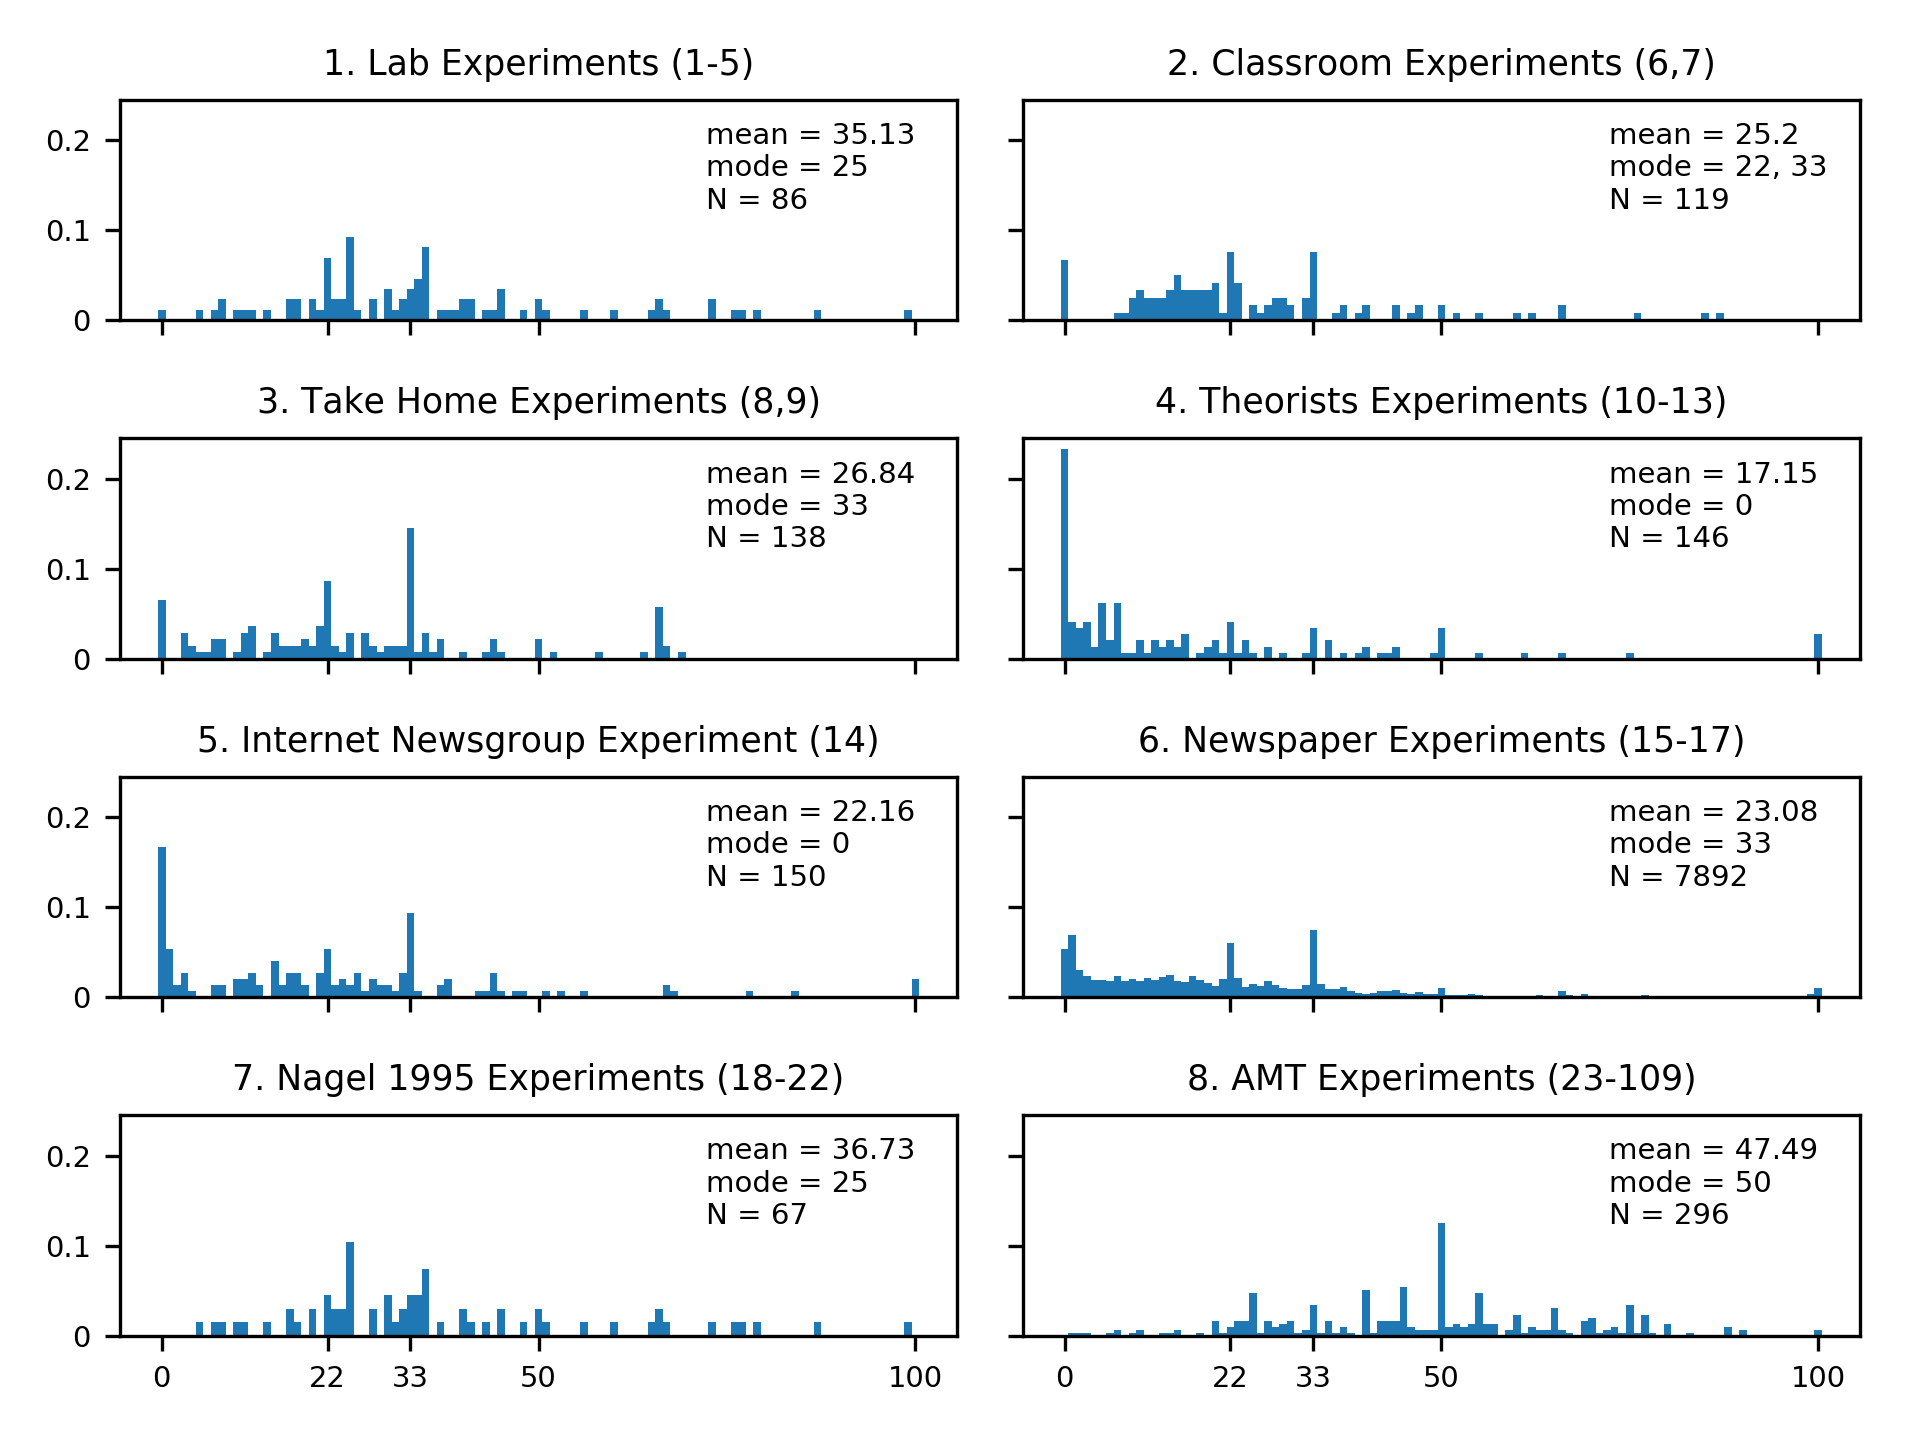
\includegraphics[width=1\textwidth]{../plots/fig1.pdf}\caption{The first six subplots show the distributions of the guesses from various ``one shot'' newspaper \cite{Thaler1997competition, selten1998zahlenwahlspiel, bosch1997juego} and lab experiments as analyzed by \citet{NagelEtAl02}. The bottom left subplot depicts the distribution of guesses in the first round in the experiments by \citet{Nagel95}, while the bottom right subplot shows the distribution of the results we collected from the first round on Amazon Mechanical Turk.}
\label{fig:all-distributions}
\end{figure}

The lowest means are found among theorists, in the internet newsgroup experiment, and in the newspaper experiments, all in which subjects were science and business interested and supposedly had more time to think about their answer and therefore may have been able to think further ahead. Specifically, the newspaper experiments were done in the magazine \textit{Spektrum der Wissenschaft} \cite{selten1998zahlenwahlspiel} (with a mean of 22.1), in the \textit{Financial Times} \cite{Thaler1997competition} (mean 18.9) and in the Spanish newspaper \textit{Expansión} \cite{NagelEtAl02} (mean = 25.5). However, another large scale experiment with 19,196 readers of the less science and business oriented Danish daily newspaper \textit{Politiken}, reported a mean of 32.4 \cite{schou2005gaet} (not shown here).

The presence of spikes in the vicinity of 22.2 and 33.3 in the majority of experiments shown in Figure~\ref{fig:all-distributions} constitutes evidence that subjects can be described as performing one or two iterations of best response reasoning. thus replicating the
findings of \citet{Nagel95}, and upholding the IBRd model as the
prominent description of how people reason about each other
and behave in the beauty contest as stated in Fact~\ref{fact:spikes}
and Fact~\ref{fact:IBRd} above. As this pattern of behavior
is found both in lab and in newspaper experiments, the data
corroborates the assumption of parallelism between the lab and the
field (newspapers), as we have seen in Fact~\ref{fact:parallelism}.

Our findings from AMT, shown in the bottom right graph of Figure~\ref{fig:all-distributions},
tell a different story. First of all, while the mass of all other
distributions is concentrated on the left half of the interval {[}0,100{]},
the distribution of the data from AMT is close to normal ($p=0.047$, Shapiro-Wilk test) with mode 50 and mean 47.49, and has mass concentrated around the center of
the interval and spreading away symmetrically in both directions.
Moreover, the three different treatments all have means above 45 (50.99
for 2-player groups, 45.42 for 4-player groups and 45.96 for 8-player
groups), and the mode is 50 for each treatment too, overall indicating
a propensity towards a middle number in the first round.

Second, unlike the other seven distributions in Figure~\ref{fig:all-distributions},
the one from AMT has no notable spike either around 33.33 or around
22.22. A major spike at 50 is instead present, which corresponds to
the modal choice, while lower spikes appear more or less symmetrically
on both sides of it. We can therefore state the following:

\begin{fdn}
No spikes confirming the effect of some iterations of IBRd reasoning are found.
\end{fdn}

%Figure~\ref{fig:cdfs} shows the cumulative distribution functions
%associated with the distributions in Figure~\ref{fig:all-distributions}.
%
%\begin{figure}
%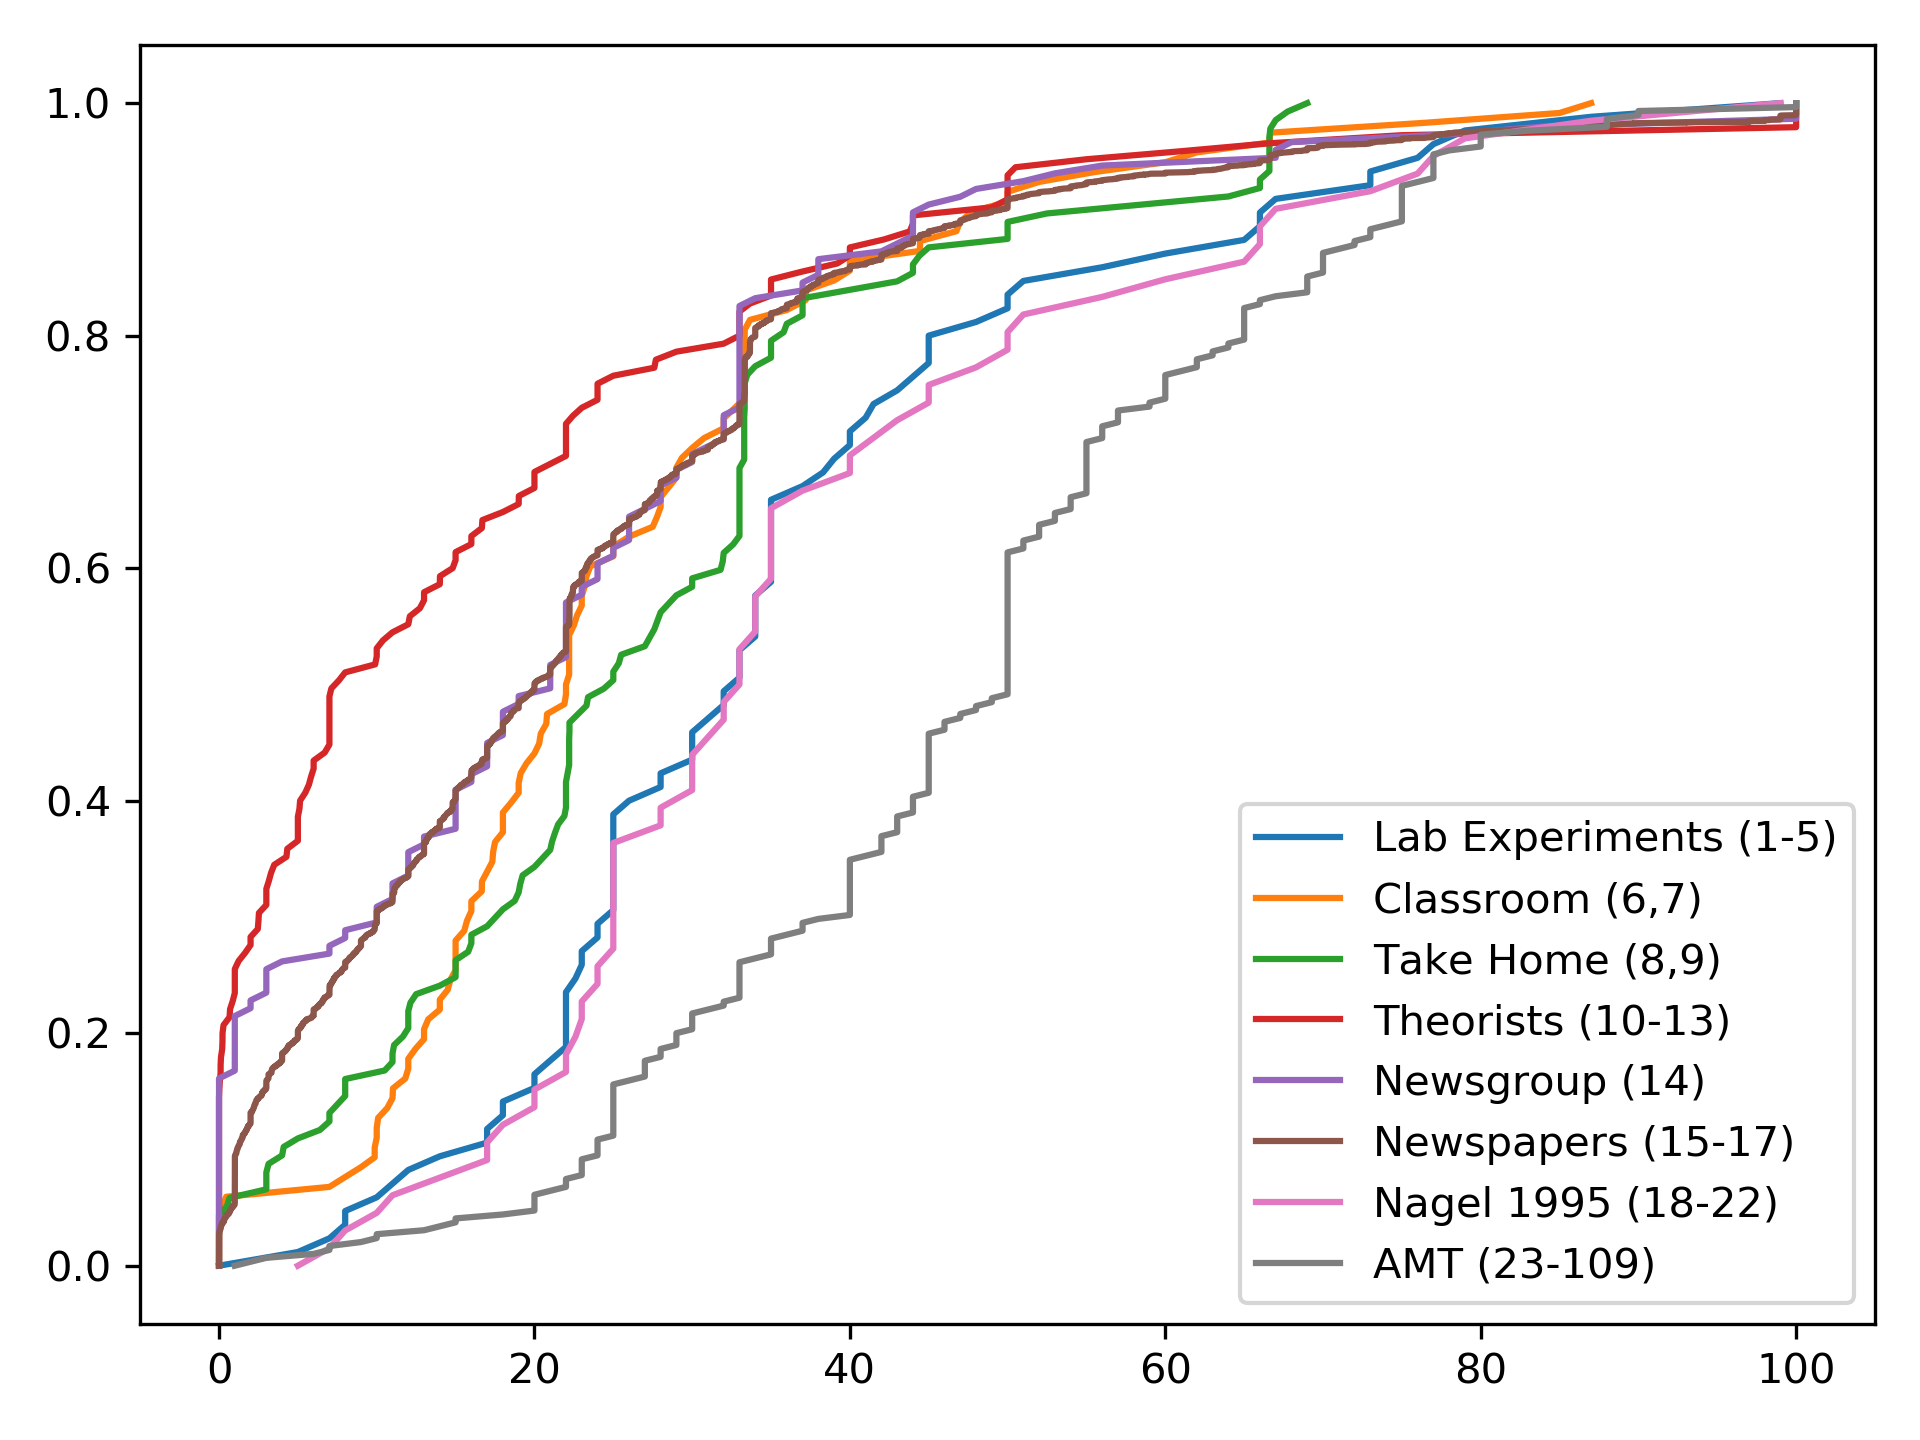
\includegraphics[width=1\textwidth]{../plots/fig2.pdf}\caption{Cumulative distributions of guesses for the 8 groups of experiments
%in Figure~\ref{fig:all-distributions}.}
%\label{fig:cdfs}
%\end{figure}

%All distributions except for the eighth brown one corresponding to
%AMT data have at least 80\% of the probability mass concentrated on
%numbers lower than 50. In the AMT case, instead, only half of the
%probability mass lies on numbers smaller than 50. 

The IBRd model assumes that the iteration process starts from 50,
as detailed previously in Section~\ref{sec:Introduction}. Such a
starting point may be interpreted as the expectation from randomly
choosing according to a symmetric distribution around 50, or as the
choice of a salient number \`{a} la Schelling \citep{sch60}. The
distribution of choices on AMT is compatible with both these hypotheses:
given the marked central spike, we can exclude that the symmetric
distribution is uniform, hence supporting some sort of salience in
the number 50. 

A second conclusion can then be drawn from our experiments: 

\begin{fdn}
The behavior observed in AMT experiments is compatible with players choosing at random from a symmetric distribution with mean 50, possibly viewed as a salient number. Relative to the IBRd model, this can be interpreted as a population of 0-level players, choosing numbers at random or by simple salience, without any higher-order reasoning.
\end{fdn}

\subsection{Dynamic: Subsequent Rounds\label{subsec:Dynamic:-Subsequent-Rounds}}
\noindent
Clear evidence for higher-order reasoning is not found in subsequent rounds either. Figure~\ref{fig:means} shows the means in each of the eight rounds played on AMT by groups of size 2, 4, and 8 respectively. For comparison we show the results of the experiments by \citet{Nagel95}, by \citet{Kamm2008unter} as reported in \cite{diekmann2009rational}, by \citet{weber2003learning}, and by \citet{buhren2010chess}, all shown in red colors.

\begin{figure}
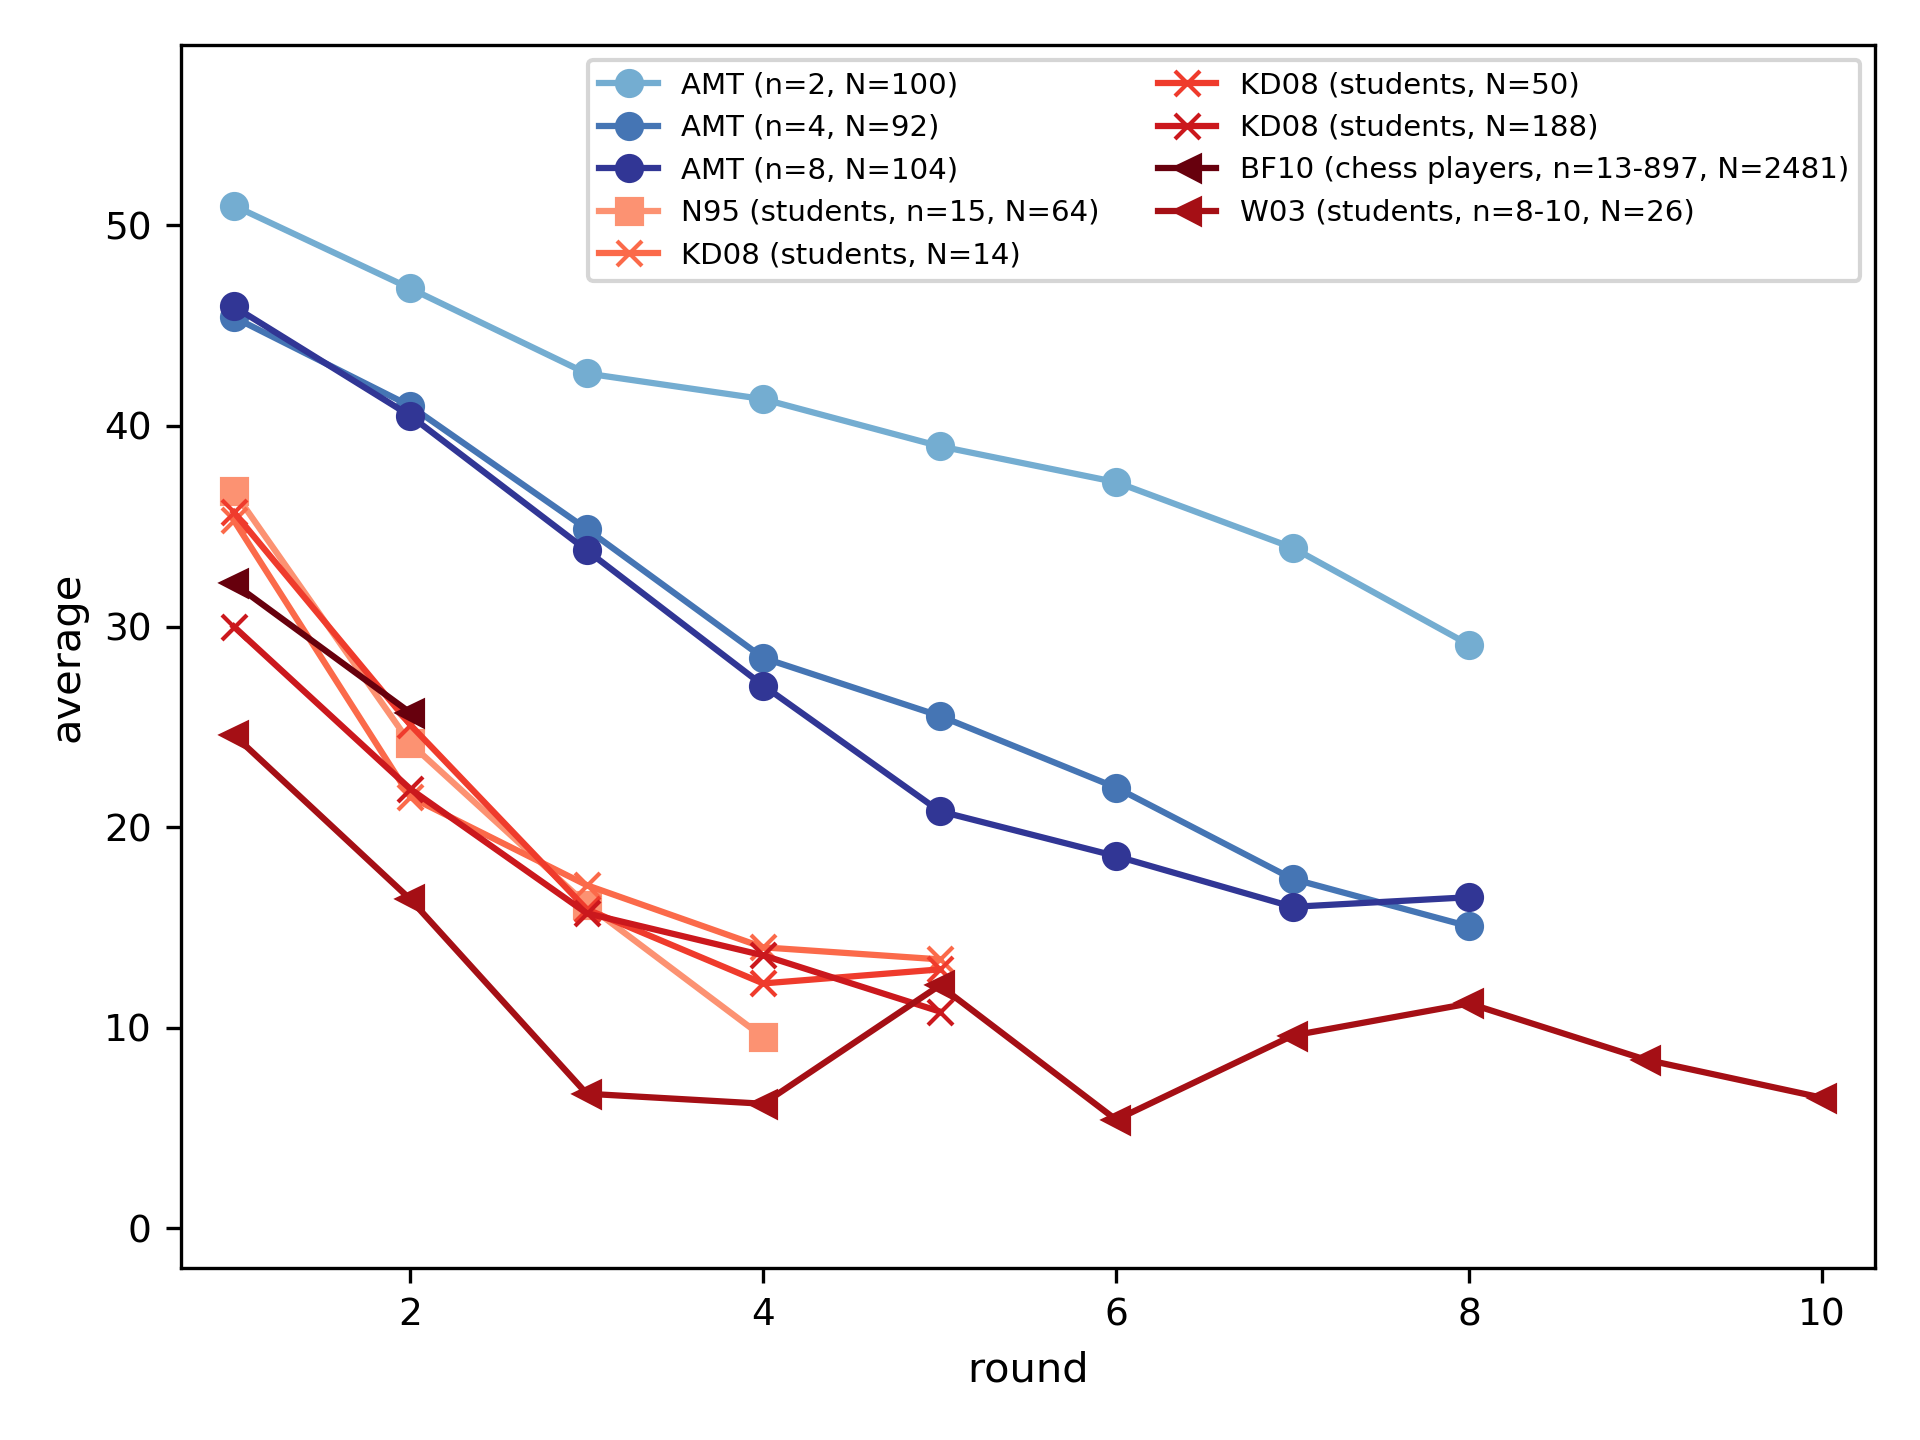
\includegraphics[width=1\textwidth]{../plots/fig3.pdf}
\caption{Means for iterated beauty contest experiments with various number of rounds played. Our AMT-experiments with group sizes 2, 4 and 8  are shown in blue colors. Results from lab experiments with students by \citet{Nagel95, Kamm2008unter, weber2003learning}, and with chess players \citet{buhren2010chess} are shown in red colors. Means decrease over time, although the AMT-results are markedly shifted upwards. In addition, the rate of decrease is significantly lower. The rates of decrease for the first four rounds in the AMT experiments are 0.19, 0.37, and 0.41 for group sizes 2, 4 and 8, respectively, while the rate of decrease in \citet{Nagel95} is 0.74.}
\label{fig:means}
\end{figure}

It is common to all the experiments in Figure~\ref{fig:means} that the means tend to decrease with subsequent rounds, which may be interpreted as a sign of learning. The speed of decrease, however, differs between
the experiments in the lab and those on AMT. \citet{Nagel95} finds a decrease of around 30 points in four rounds. It takes instead eight rounds on AMT for the means of 4- and 8-player groups to decrease by about the same, while the means of 2-player groups decrease only by around 20 points over eight rounds.

The rates of decrease of the means between round 1 and round 4 may be computed, as in \citet{Nagel95}, by the following formula:
\[
\text{Rate of decrease}=\frac{(\text{mean}(1)-\text{mean}(4))}{\text{mean}(4)}
\]
where $\text{mean}(r)$ is the mean in round $r$. The rate of decrease in the various experiments is listed in table \ref{table:1}:

\begin{SCtable}
\begin{tabular}{lccc}
\hline
Experiment   &  n 		&  N 	&  RoD \\
\hline
Amazon Mechanical Turk   & 2 		& 100 	& 0.19 \\
	   & 4 		& 92 	& 0.37 \\
	   & 8 		& 104 	& 0.41 \\
Nagel (1995)    & 15-18 	& 64  	& 0.74  \\
Kamm \& Dahinden (2008)  & 14 		& 14 	& 0.60  \\
	   & 50 		& 50 	& 0.66  \\
	   & 188 		& 188 	& 0.55  \\
Weber (2003)   & 8-10	& 26	& 0.75  \\
\hline
\end{tabular}
\caption{Rates of decrease in iterated p-beauty contest experiments with $p=2/3$. n = group size; N = number of subjects; RoD = rate of decrease from round 1 to round 4.}
\label{table:1}
\end{SCtable}

As it can be seen from table \ref{table:1}, the rate of decrease of the mean in our AMT experiment are much lower than in all the other experiments done on students, which leads us to make the following finding:


\begin{fdn}
The means of all treatments in the AMT experiments are significantly higher than the means of the experiments in \citet{Nagel95, Kamm2008unter} and \citet{weber2003learning}. Moreover, the rates of decrease of the means in all treatments from AMT experiments are substantially lower than the rate of decrease in the repeated beauty contest experiments by \citet{Nagel95, Kamm2008unter} and \citet{weber2003learning}.
\end{fdn}

In addition, the means in 2-player groups are significantly higher than in 4-player and 8-player groups (Kolmogorov-Smirnov tests, $p<0.01$ in 14 out of 16 comparisons), indicating that when playing against
only one player, people behave differently. As already noticed in \citet{HoCamererWeigelt98}, this is puzzling in that the smaller the group, the larger the effect of individual guesses on the mean. Two-person beauty contests are isomorphic to the game \textquotedblleft whoever chooses the smaller number wins\textquotedblright : while one is not
guaranteed to win when choosing zero in the 4- or 8-player beauty contest, guessing zero is weakly dominant and ensures at least a tie in the 2-player game. 

In our 50 experiments with groups of two players, there was no participant who chose zero in the first round. After
8 rounds, zero was chosen 3 times in total (out of 800 guesses). This is significantly lower than what was found previously by \citet{NagelGrosskopf2008}, where about 10\% of undergraduates in economics guessed zero in the one-shot version of the 2-player game.

Finally, higher rates of decrease are sometimes associated with larger groups (e.g. \citet{HoCamererWeigelt98}, p. 958), but the similarity in the means between groups of 4 and 8 players and the comparison to the results by \citet{ Kamm2008unter} and \citet{weber2003learning} both have comparable group sizes constitute counterexamples to that association. AMT experiments also contradict the claim that larger groups choose higher numbers at the start (see \citet{HoCamererWeigelt98}, p. 958). What holds true, instead, is that the 2-person beauty contest constitutes a puzzling case in which the players not only lack the strategic sophistication to understand the great power in their hands, but even display a tendency towards higher guesses than in groups with more than two players. A possible explanation, also suggested by \citet{NagelGrosskopf2008}, may be based on a cognitive misconception of the game: players might aim to be as close as possible to the $2/3$ of the mean rather than to be clos\emph{er} than the opponent to the $2/3$ of the mean. We can thus state the following:

\begin{fdn}
On average, participants in the 4-player and 8-player treatments guess significantly lower than in the 2-player treatment. Moreover, the rates of decrease of the means in the 4-player and 8-player treatments are significantly higher than the rate of decrease in the 2-player treatment.
\end{fdn}

It is noticeable that simple directional learning also seems to be
falsified by AMT experiments. Figure~\ref{fig:above-2/3} pictures
the distribution of the number of times a player chooses a number
greater than the target of the previous round, i.e., greater than
$2/3$ of the previous mean. Experiments on AMT, on the right, show
that less than 2\% of players never guess higher than the target of
the previous round, while the vast majority (more than 80\%) does
that at least three times, and about 50\% does it five times or more.

\begin{figure}
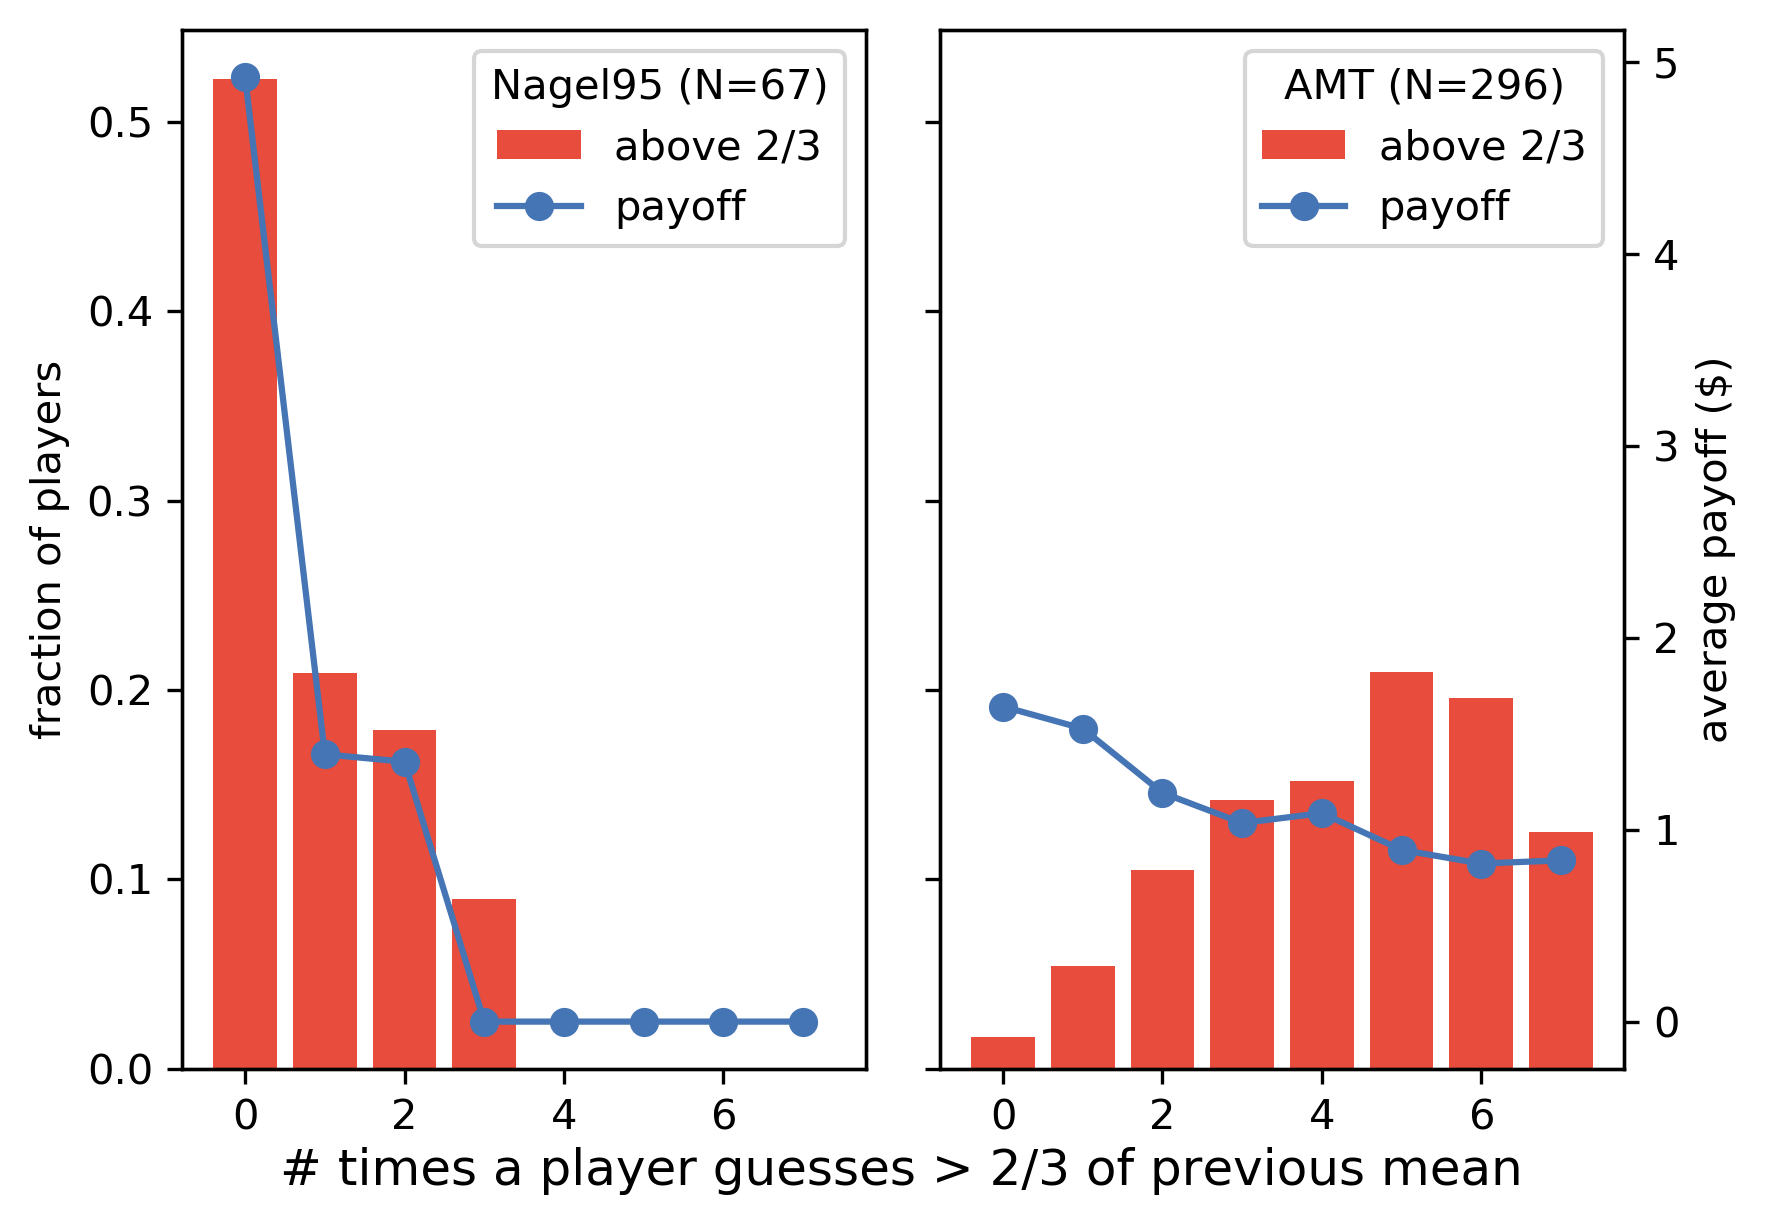
\includegraphics[width=1\textwidth]{../plots/fig4.pdf}
\caption{Bar chart of the number of times a player chooses a number greater
than $2/3$ of the mean of the previous round. In the lab experiments
by \citet{Nagel95} (left) 52\% of the players never go above $2/3$
of the previous mean, and only about 25\% do that more than once.
In the AMT experiments (right) less than 2\% of players never go above
$2/3$ of the previous mean, while 53\% of players go above $2/3$
of the previous mean more than four times.}
\label{fig:above-2/3}
\end{figure}

The distribution on the left, corresponding to the lab experiments
by \citet{Nagel95}, depicts players of a different kind: more than
50\% of players never go higher than the target of the previous round,
while only about 25\% do that more than once. Importantly, both in
the lab experiments by \citet{Nagel95} and in the experiments on AMT,
at the end of each round players were told both the mean and the two-thirds
of the mean of that round, as well as all chosen numbers.%
{} While the players in \citet{Nagel95} seem to learn that the target
decreases and adapt to this, players on AMT cannot be viewed as adapting
to a decreasing target: most of the times they pick numbers higher
than $2/3$ of the mean of the previous round, even while observing
a decreasing sequence of means and targets.

From the assumption that, in subsequent repetitions, a player of level
zero chooses at random according to a symmetric distribution around
the previous mean (or the previous target), it follows that a player
of level one would never guess higher than the previous target, and
higher levels of reasoning imply even lower guesses. Hence, the combination
of some iterations of IBRd with an adaptation process taking the mean
(or two-thirds of the mean) of the previous round as reference point
for the next round is incompatible with our observations from AMT.
We can therefore state the following:

\begin{fdn}
The results from the AMT experiments are incompatible with the combination of higher-order reasoning as modeled by IBRd and learning processes taking the mean (or two-thirds of the mean) of the previous round as the reference point for the next round. 
\end{fdn}

\section{Parallelism between the Field and the Lab\label{sec:Parallelism}}
\noindent
In light of the results above, we have to reassess the assumption
of parallelism between the lab and the field. Participants in lab
and classroom experiments are most often university students, sometimes
even graduate or PhD students in economics, and hence cannot be considered
representative of the population at large. As mentioned in Section~\ref{sec:Introduction},
this causes issues about the sociodemographic representativeness of
such samples: how general and generalizable are the results from the
lab? So-called field experiments such as newspaper experiments, on
the other hand, may potentially reach broader and more differentiate
subject pools, but at the price of losing control on the specific
sociodemographic characteristics of the sample.

One of the important contributions by \citet{NagelEtAl02} concerns
the parallelism between the lab and the field. Accepting the experiments
with newspaper readers as field experiments, the comparison between
the results from newspaper and lab/classroom experiments allows the
authors to evaluate the assumption of parallelism and the general
validity of the conclusions drawn from lab behavior. Given the similarity
between the data collected from newspaper experiments and those from
various lab and classroom experiments, \cite{NagelEtAl02} conclude
that the same pattern observed in the three newspaper experiments
is replicated in the lab, and the parallelism assumption between the
lab and the field is supported, as we have seen in Fact~\ref{fact:parallelism}.

The sizable differences reported above with respect to the behavior
in online experiments on Amazon Mechanical Turk would lead us to the
opposite: 

\begin{fdn}
In our AMT experiments, the parallelism between the lab and the field fails.
\end{fdn}

\section{Conclusion: A Dilemma\label{sec:Conclusion}}
\noindent
The main conclusions drawn by \cite{NagelEtAl02} on the assumption of parallelism and the common behavioral patterns observed both in lab and in field (newspaper) experiments are thus not supported by our results from AMT. Similarly to the newspaper experiments, AMT experiments reach broader and more differentiate pools than lab experiments \citep{BuhrmesterEtAl2011,CrumpEtAl13,HortonEtAl2011,Rand2012}, but also have less control on the sociodemographic characteristics of the sample. As opposed to lab experiments, AMT experiments are
thus to be considered field experiments. 

Putting these two observations together leaves us with a dilemma. Either AMT is not a reliable platform for small and medium sized beauty contests, or the assumption of parallelism between the lab and the field (AMT) does not hold true. 

In the first case, our results would contradict the literature about the validity of experiments performed on AMT (e.g. \cite{BuhrmesterEtAl2011,CrumpEtAl13,HortonEtAl2011,Rand2012}). In the second, they would go against the validation of parallelism between the lab and newspaper experiments as investigated by \cite{NagelEtAl02}. 

Arguments for the first case may include the belief that the quality of the AMT subject pool is poor in terms of monetary incentives, attention and/or cognitive ability and effort. However, the average payoff in our experiments was approximately \$15 per hour, which is considered generous according to AMT guidelines and certainly above the estimated average of \$6 per hour when excluding un-submitted and rejected work \citep{HaraEtAl18}. In addition, the belief that data quality depends on the (relative) size of the bonus compared to the participation fee is contradicted by \cite{amir2012economic}, who showed that results of standard economic games with very low bonuses on AMT are comparable to those of corresponding lab experiments with higher bonuses, thus alleviating concerns about the validity of economic game experiments conducted on AMT. 

With regard to possible concerns about insufficient cognitive ability and/or effort among AMT subjects, we can only suggest that in order for economic games to be representative of the real world, they should not require subjects to be experts or be trained in any particular way. If the keynesian beauty contest were meant to test the cognitive acumen of only economists and mathematically talented people, it is clear that AMT is not the best place to do such experiments. If, however, the purpose of the p-beauty contest is to say something general about people's use of higher-order reasoning in online settings, AMT may be a good place to start. 

However, the apparent lack of strategic thinking among the majority of AMT subjects is still a puzzle which needs further investigation. As discussed in \citet{chou2009control} one reason may be may be that the beauty contest is an unfamiliar type of game in which subjects often lack understanding of the relationships between possible choices, outcomes and payoffs. Online platforms like Amazon Mechanical Turk, where subjects have no prior knowledge, limited time and little patience, may amplify such contributing factors. When instructions and procedures are presented with mathematical expressions like ``average'' and ``2/3 of'', subjetcs may believe that they are supposed to solve mathematical problems rather than to think about what others think. Our two-person beauty contest experiment may be a glaring example of such misconceptions. If the instructions were presented in a more familiar context and with a clear statement such as ``whoever chooses the lowest number wins'', strategic thinking would probably have been more prevalent \cite{chou2009control, bosch2019one}.

To conclude, the differences between our results and the results from newspaper/lab experiments are most likely due to the disparities between their subject pools. Consquently we conjecture that the similarity between newspaper and lab results may be due to the similarity between their subject pools. Although it is true that the design of the newspaper experiments entails a loss of control on the sample, it does not necessarily follow that the newspaper samples are very different and more diverse than the samples used in lab experiments. Having chosen markedly economic-oriented newspapers might have brought the experimenters not very far into the field. Further lab, field and AMT experiments that control for some of the factors discussed above should be able to answer the dilemma presented here.

\bibliography{gor}  

\newpage
\appendix
\setcounter{page}{1}
\title{Supplementary Material for the article ` Strategic Reasoning Online: Experiments on the Beauty Contest'}
%\maketitle

\section{Materials and Method}
Amazon Mechanical Turk (AMT) is an online labor market and crowdsourcing platform, which is increasingly being used for social and economic experiments in order to investigate the real time interactions of small to medium sized groups. AMT has repeatedly been shown to meet or exceed the standards set by data collection methods using other means \citep{berinsky_huber_lenz_2012, BuhrmesterEtAl18}. The platform has a large participant pool (called turkers), various demographic and quality selection options for researchers, and provides an integrated participant compensation system.

\section{Experimental Design}
After turkers accept our ‘HIT’ (‘human intelligence task’), they have to provide informed consent, see Figure \ref{Fig S1}. Then they wait until there are enough turkers who have accepted the HIT to form random groups (grouped by arrival) of size 2, 4 or 8, respectively, depending on the treatment condition. 
When group has been formed, instructions are displayed for 90 seconds, see Figure \ref{Fig S2}. After pressing NEXT, turkers see a page where they have to enter into a form field an integer number between 0 and 100. When all turkers in a group have done so, a result page is displayed, see Figure \ref{Fig S3}, where they can see their own guess, the guesses of the other players, the average and the 2/3 of the average as well as information about whether they have won a bonus in the current found and what their total payoff is for the time being. 
After this, the previous steps are repeated for a total of 8 rounds. Every time turkers enter a new number, they can see a list of the 2/3 of the average of the previous rounds as shown in Figure \ref{Fig S4}. Turkers have 90 seconds to think about a number. After eight rounds, turkers are required to give feedback by answering the question: ‘What strategy did you use while playing this game?’, after which they are thanked for their participation.

\begin{figure}
\includegraphics[width=1\textwidth]{../images/FigA1.png}\caption{Screen dump of the consent page shown to all participants.}
\label{Fig S1}
\end{figure}

\begin{figure}
\includegraphics[width=1\textwidth]{../images/FigA2.png}\caption{Screen dump of an instruction page for a game with four players.}
\label{Fig S2}
\end{figure}

\begin{figure}
\includegraphics[width=1\textwidth]{../images/FigA3.png}\caption{Screen dump of a result page from a game with four players.}
\label{Fig S3}
\end{figure}

\begin{figure}
\includegraphics[width=1\textwidth]{../images/FigA4.png}\caption{Screen dump of a choice page from a game with four players.}
\label{Fig S4}
\end{figure}

\section{AMT Setting}
When working with AMT it is important to consider the right settings in order to get the best data quality possible \citep{ChandlerShapiro16}. Fair wage, attrition rates, removal of duplicate workers and informative feedback are some of the most important issues to address.
Average wage for turkers in our experiments was approximately \$15 per hour, which is considered generous according to AMT guidelines and certainly above the estimated average of \$6 per hour when excluding un-submitted and rejected work \citep{HaraEtAl18}.
Quitting a study before completing it is prevalent on AMT, and varies systemically across experimental conditions. Our overall attrition rate was 24\%, which is considered normal \citep{ZhouFishbach16}. The main reason, we believe, was either a player not being able to enter a number within the allotted time, or – more likely – due to a player not bothering to wait for the others to make their guess and therefore quitting prematurely. This was very detrimental for the rest of the group and for the experiment as such, because it meant that the rest of the group would continue the game with one player less, making the whole process much slower and skewing the results. If somebody had quit, we still let the other players finish their game and paid them for their efforts, but we decided to remove those groups from the data analysis. Out of a total of 114 initial groups, 27 groups were thus removed from the final data set, giving an overall attrition rate of 24\%.
All turkers automatically received a unique qualification when accepting a HIT, ensuring that they could not play the game twice. In addition, we set the qualification that workers should have completed at least 50 HITs and have an accepted HIT rate of 90\% or above. This ensured that we would get experienced and qualified workers. During our experiments, participants had easy access to our email for questions and possible bug reports. 

\section{Code and Software}
All experiments are coded in the experimental software oTree 1.4.39 \citep{ChenSchongerWickens16} which is based on Python and Django. The code for the data analysis done is available on Github at https://github.com/gavstrik/game-of-regret.

\section{Data Collection and Distribution}
We obtained a total of 2368 guesses from 296 unique participants who played the classic iterated beauty contest game. Players were partitioned into 50 groups of size 2, 23 groups of size 4, and 13 groups of size 8.


\begin{figure}
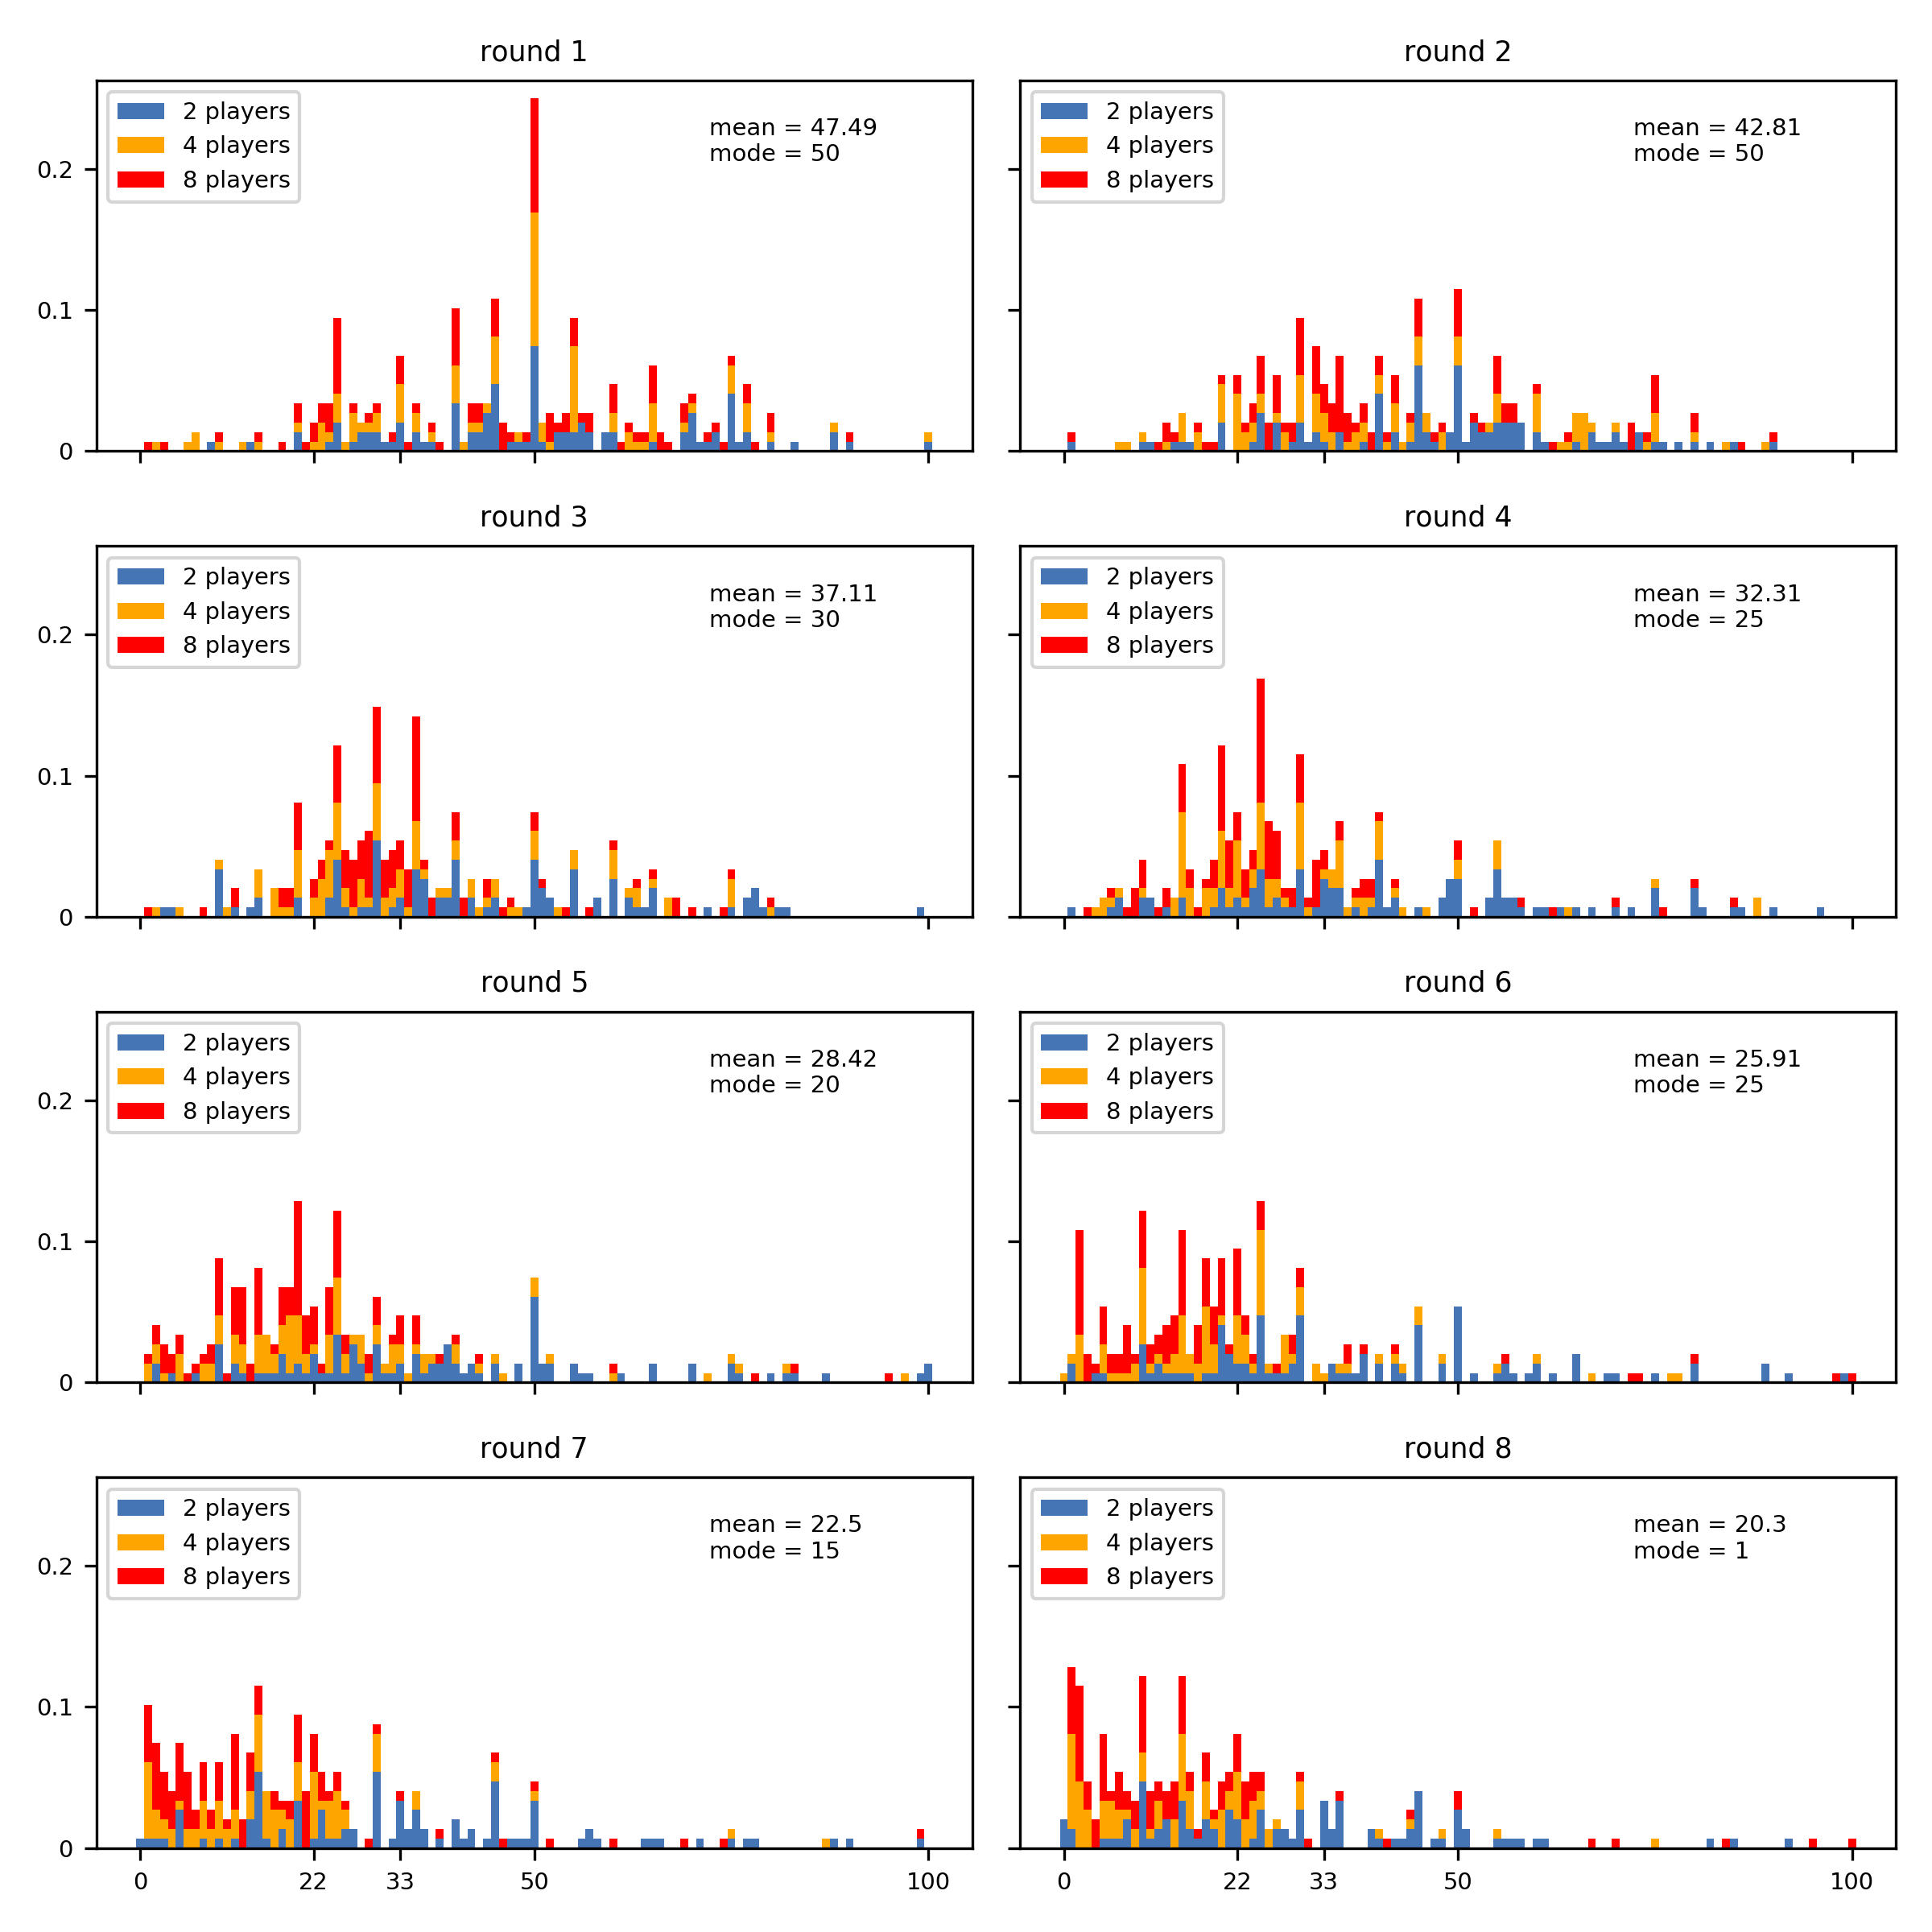
\includegraphics[width=1\textwidth]{../plots/figA5.pdf}\caption{Histograms of guess distributions partitioned into groups and rounds.}
\label{Fig S5}
\end{figure}

Figure \ref{Fig S5} shows the guesses for all eight rounds, partitioned into their respective groups. As can be seen from the histograms, guesses move slowly towards lower numbers in subsequent rounds, with the 2-players groups (in blue) lacking slightly behind the other groups.

\section{Guess Dynamics}
As noted in figure 4 in the main text, players often choose numbers greater than 2/3 of the mean of the previous round. Less than 2\% of all players on AMT never go above 2/3 of the previous mean, while 53\% go above this target more than four times. 

%Figure \ref{Fig S6} shows some examples of the up and down movements of individual guesses from one round to the next. It is difficult to interpret this behavior observed in Fig. S6 as simple directional learning. Instead, players seem to try to “talk” with each other with occasional high guesses, and instead of adapting to the new target (explicitly shown as 2/3 of the previous mean), they may adapt to what they think the other players will guess in the next round.
%
%\begin{figure}
%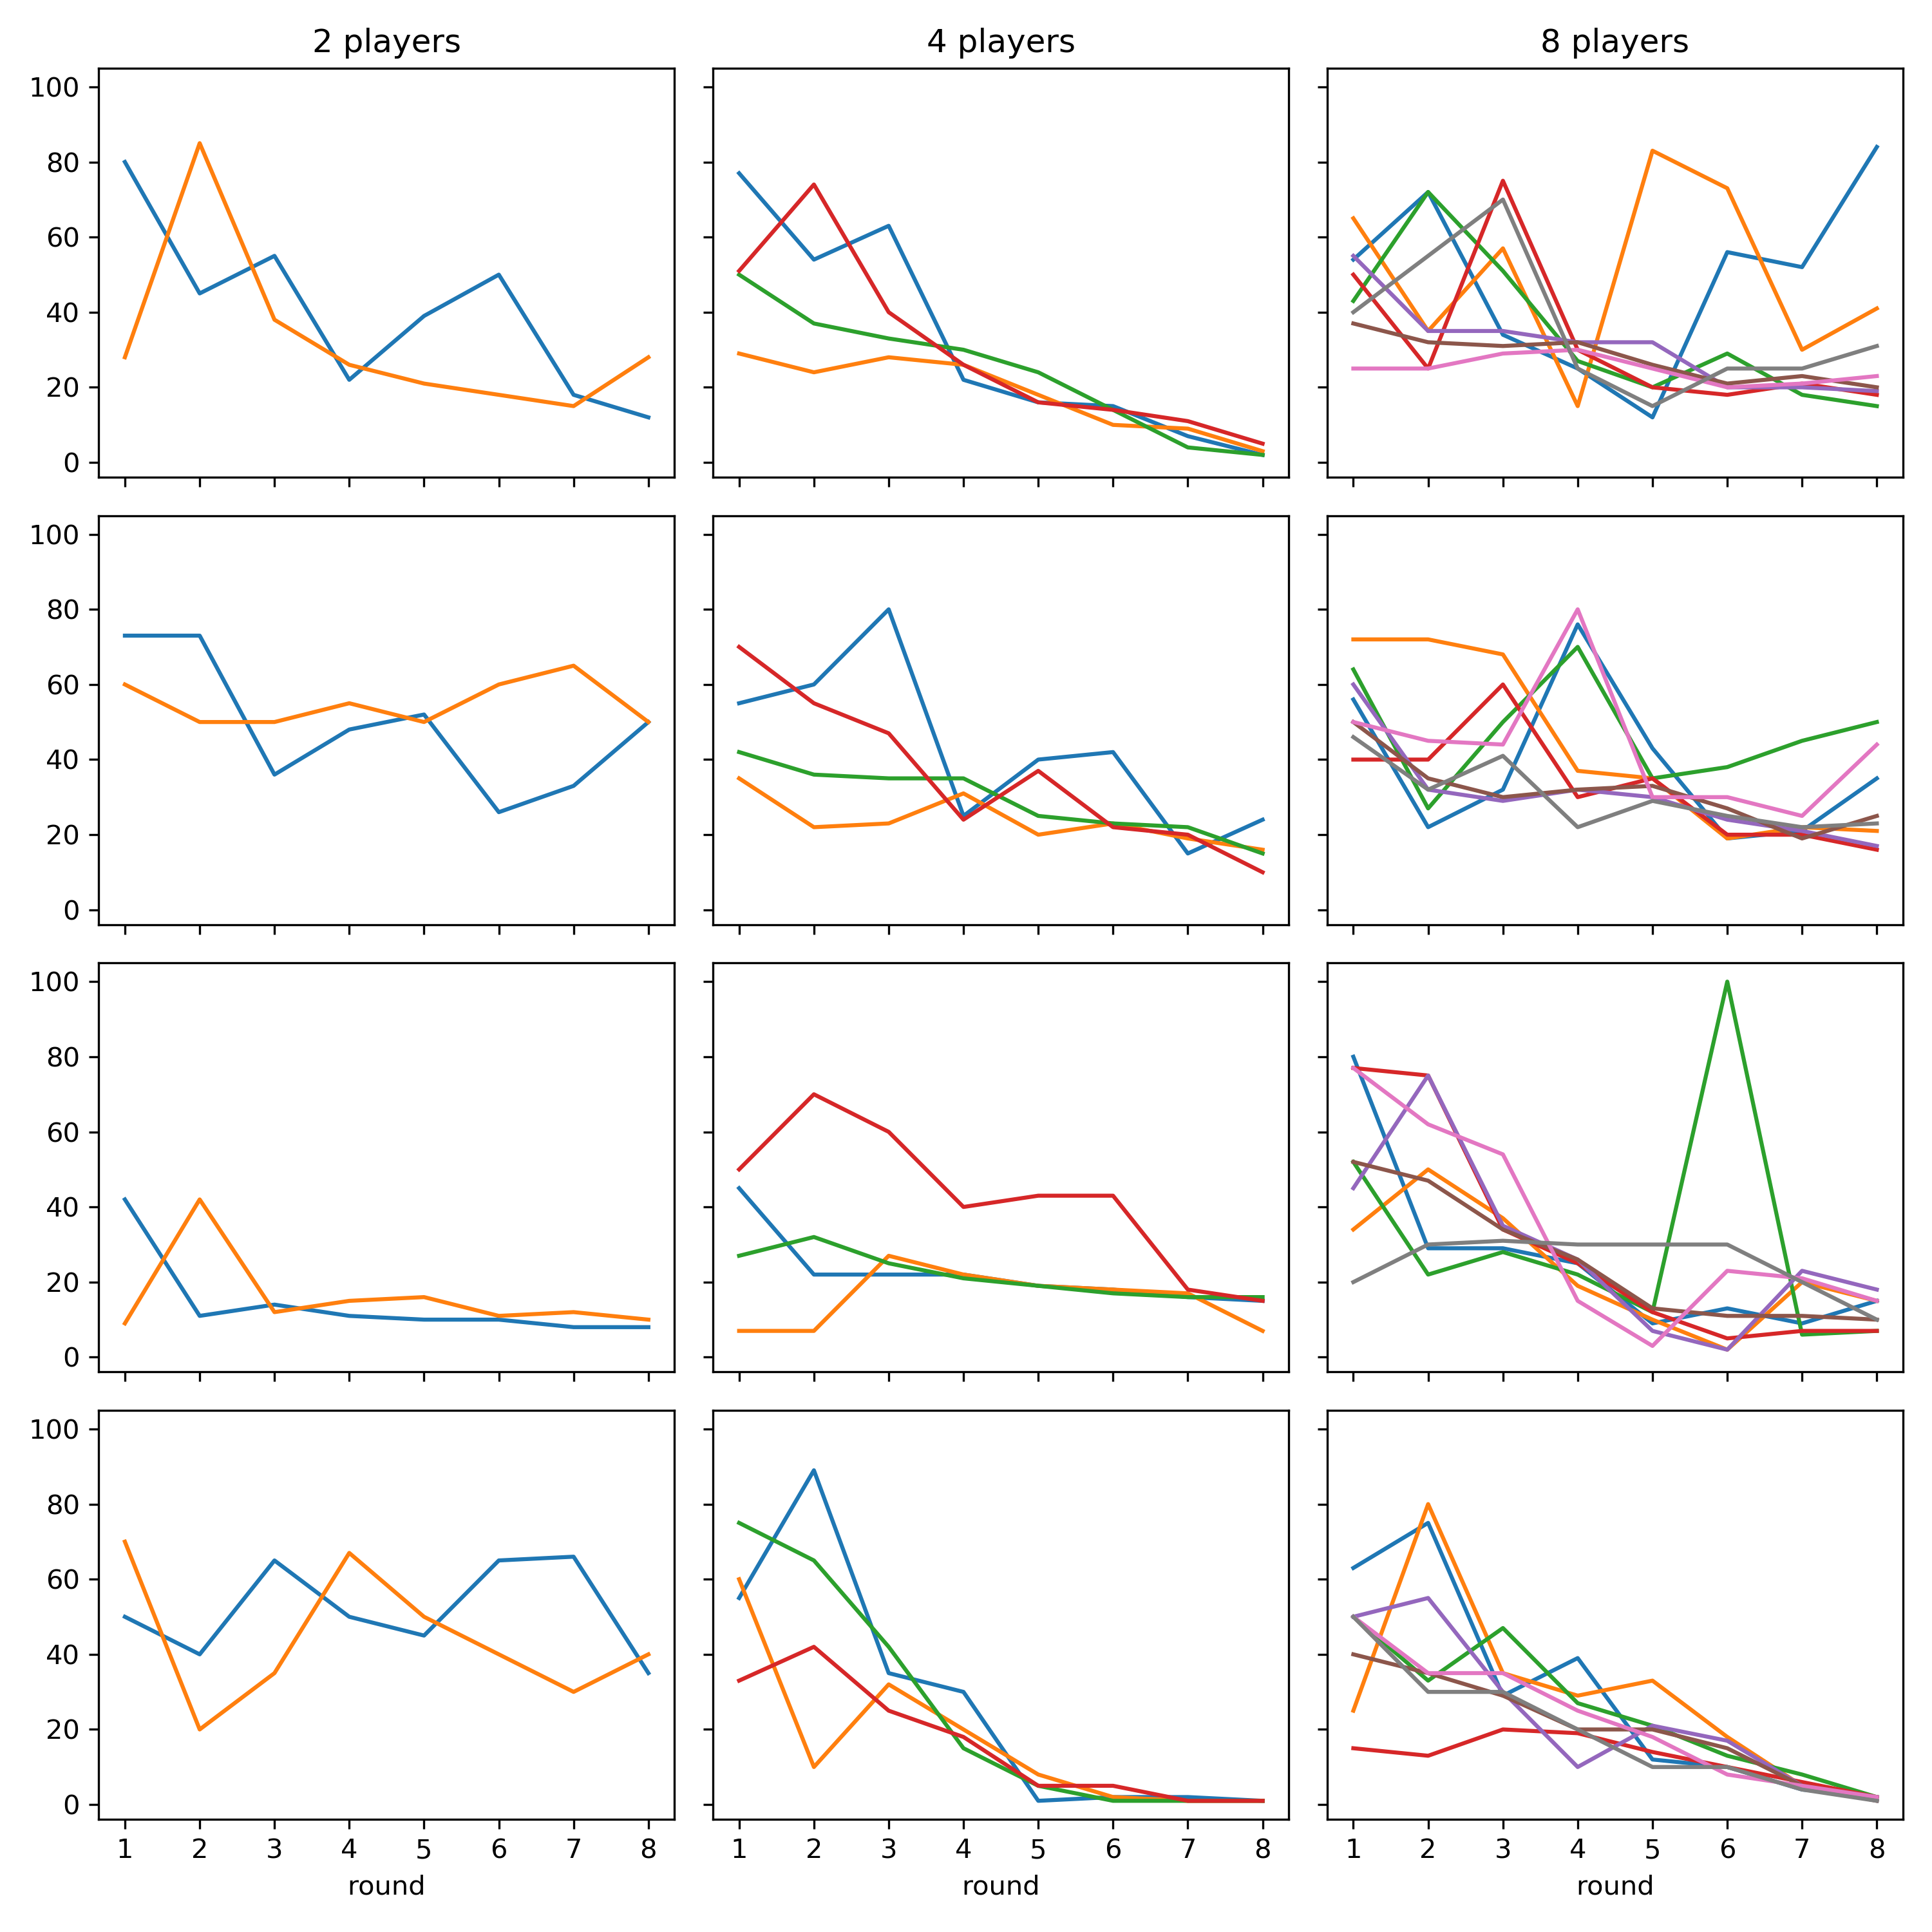
\includegraphics[width=1\textwidth]{../plots/figA6.pdf}\caption{Guess dynamics of player guesses from randomly selected groups.}
%\label{Fig S6}
%\end{figure}
%
%We can illustrate the guess-dynamics in another way as well. 
Figure \ref{Fig S7} shows the dynamics of guesses round by round in such a way that the previous round n is always shown on the x-axis and the next round $n+1$ is always shown on the y-axis. The diagonal black line corresponds to staying at the same guess in subsequent rounds. Lines connecting the dots in Figure \ref{Fig S7} then indicate the sequence of guesses by the same player, whose comments are shown in the legend. The total bonus earned is shown in parenthesis.

\begin{figure}
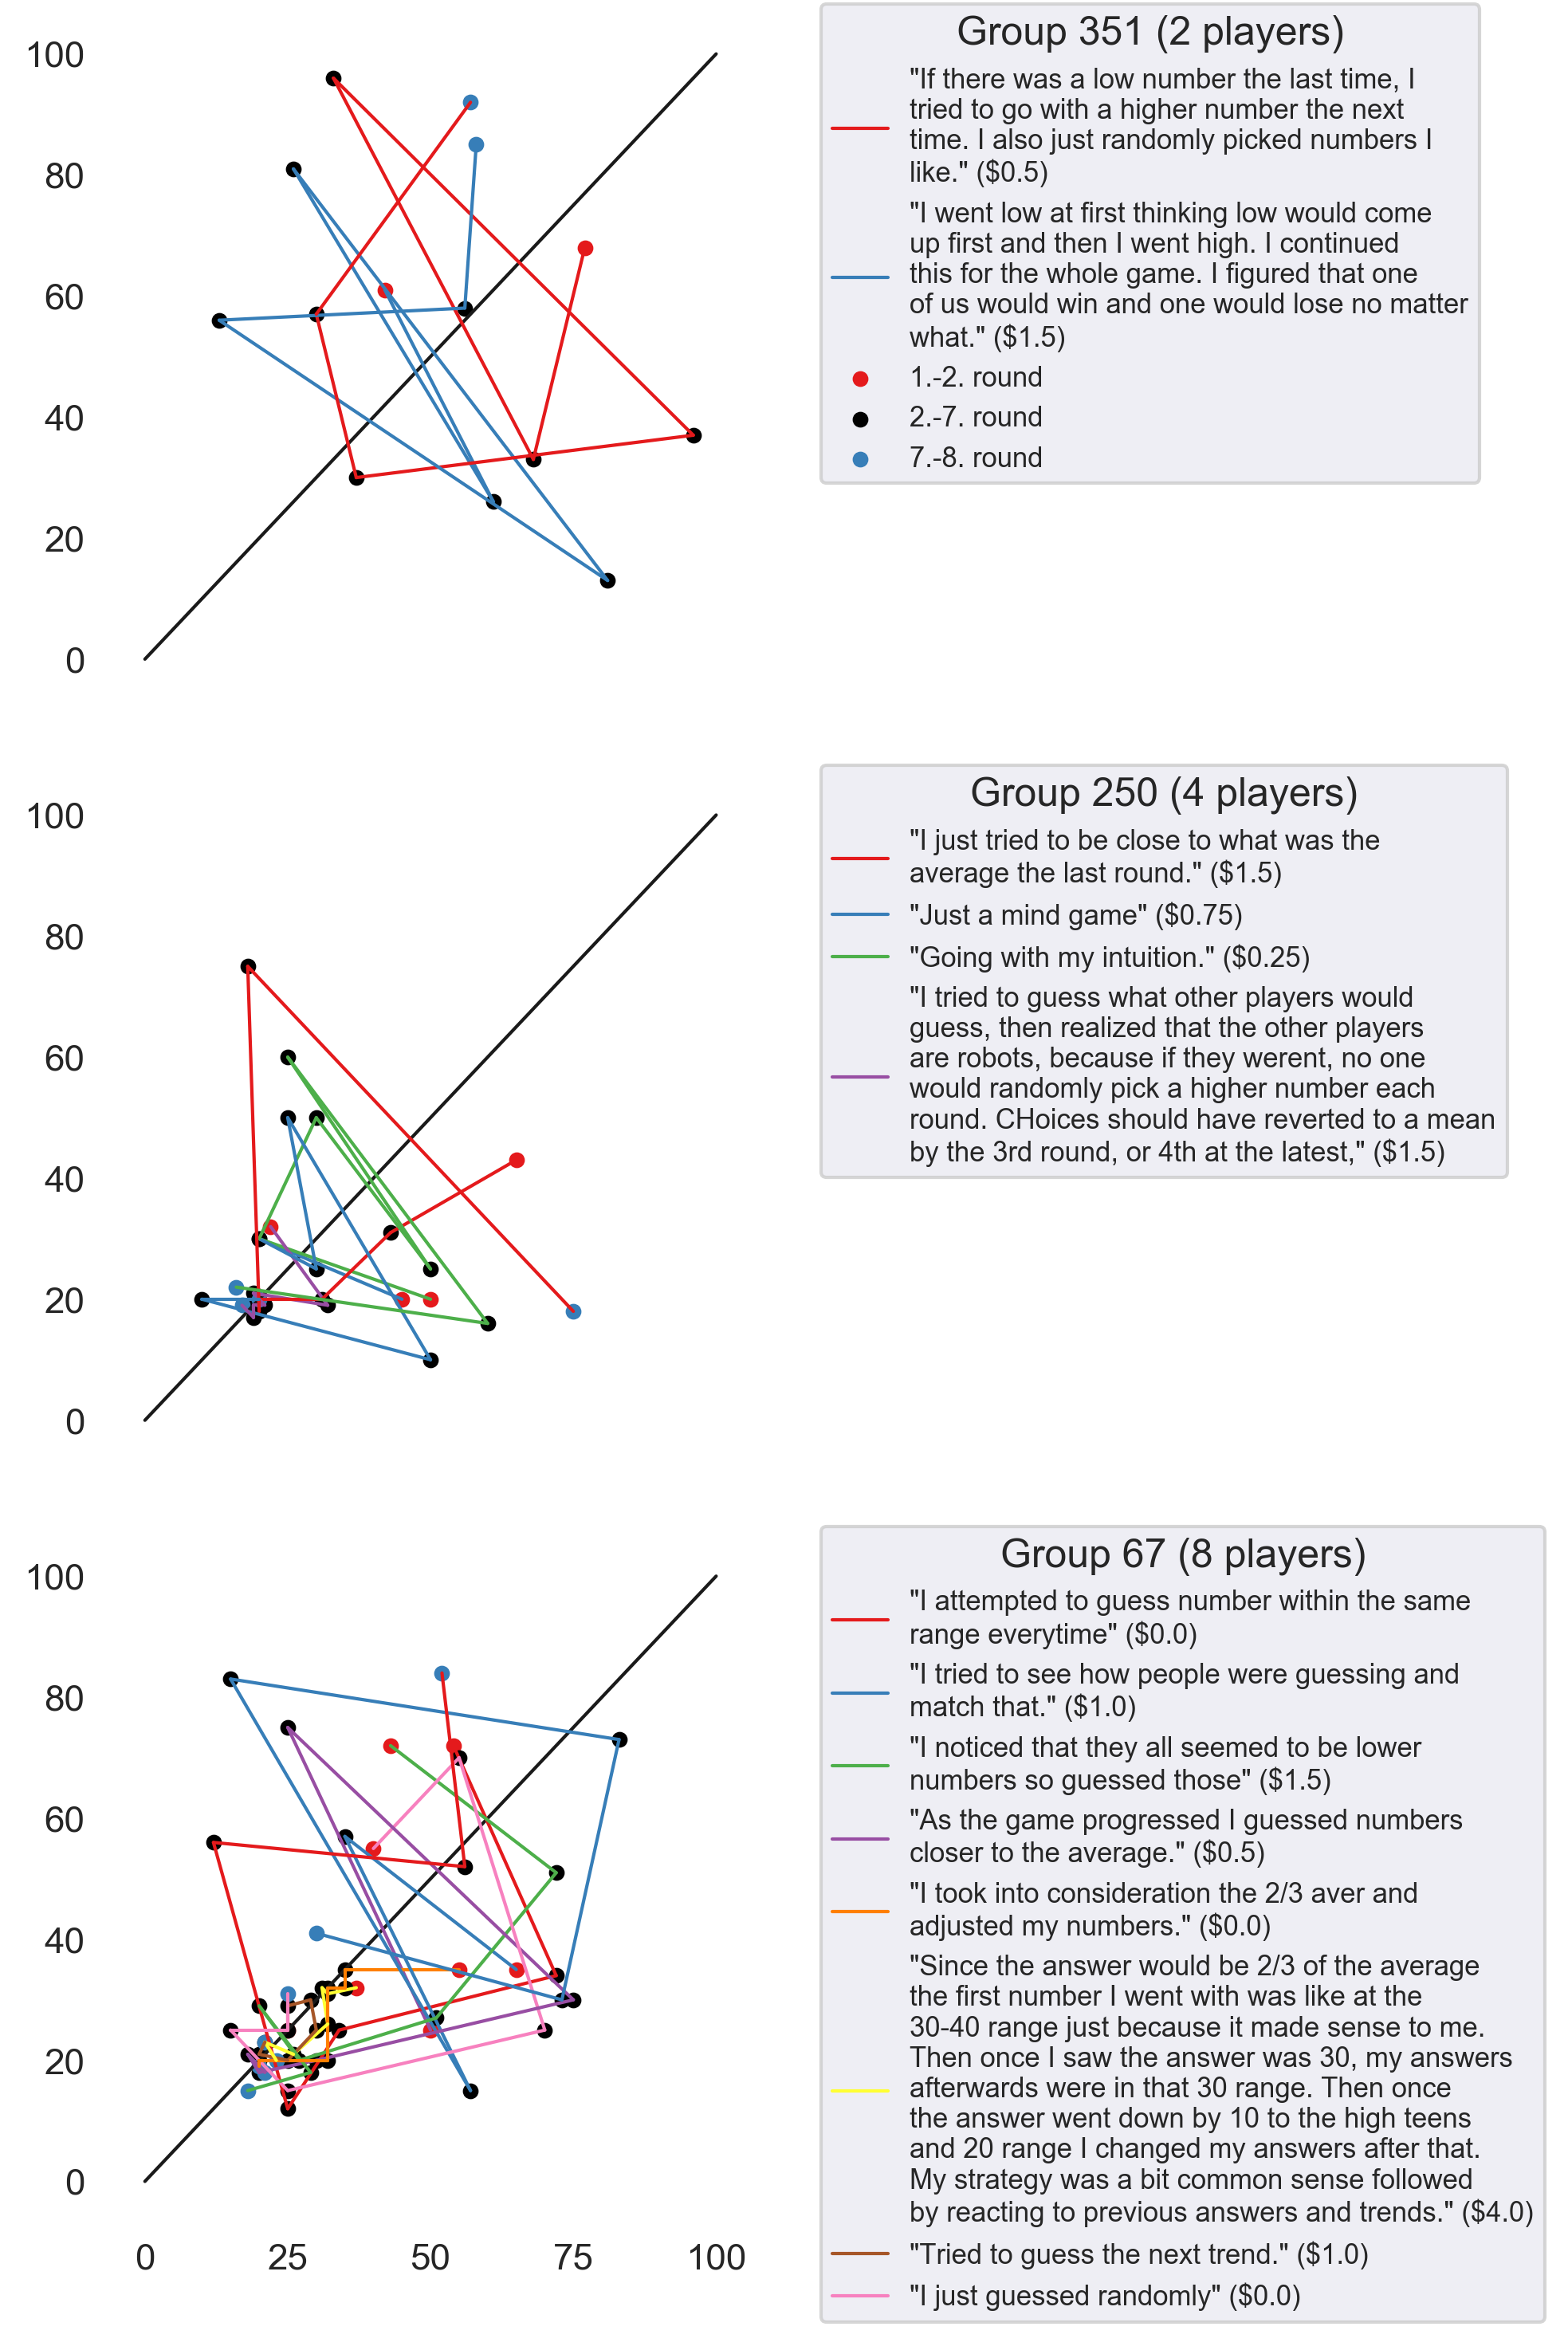
\includegraphics[width=1\textwidth]{../plots/figA7.pdf}\caption{Dynamics of guesses round by round.}
\label{Fig S7}
\end{figure}



\end{document}